\chapter{Case Study}
\todo{I don't like the name case study, since it is not really a study. What about initial evaluation? self evaluation? merge with previous chapter and make it a section?}

\todo{first general showcase from icra paper (does not have the plot widget in the screenshots), then how to add a new widget --> plot widget. Then the more specific audio source localization / sound localization showcase with nao}

\section{Visualizing Existing Data}
Although the current implementation is a prototype, it has all the features that were initially planned. The implementation is running stably and first attempts to use it as a debugging tool have been made. ROSDashboard is ready to be used for the development of robot applications and can be used for further evaluations (see Section~\ref{future_work}).

Figure~\ref{showcase} shows a simple showcase scenario: ROSDashboard is running alongside the \emph{turtlesim\_node} node which is used in many examples in the ROS tutorials\footnote{http://www.ros.org/wiki/ROS/Tutorials}. It monitors the values for linear and angular speed which are published by the \emph{turtle\_teleop\_key} node to control the turtle simulation. The String widget is configured to display messages from \emph{/rosout}, which in this example shows a warning when the turtle hits a wall.
For the purpose of this small showcase, there was no need to modify the turtlesim source code. The only topics used by the showcase scenario are topics that are already used to control the turtle in the simulation and to display warnings.

\begin{figure}[thpb]
  \centering
  \framebox{
    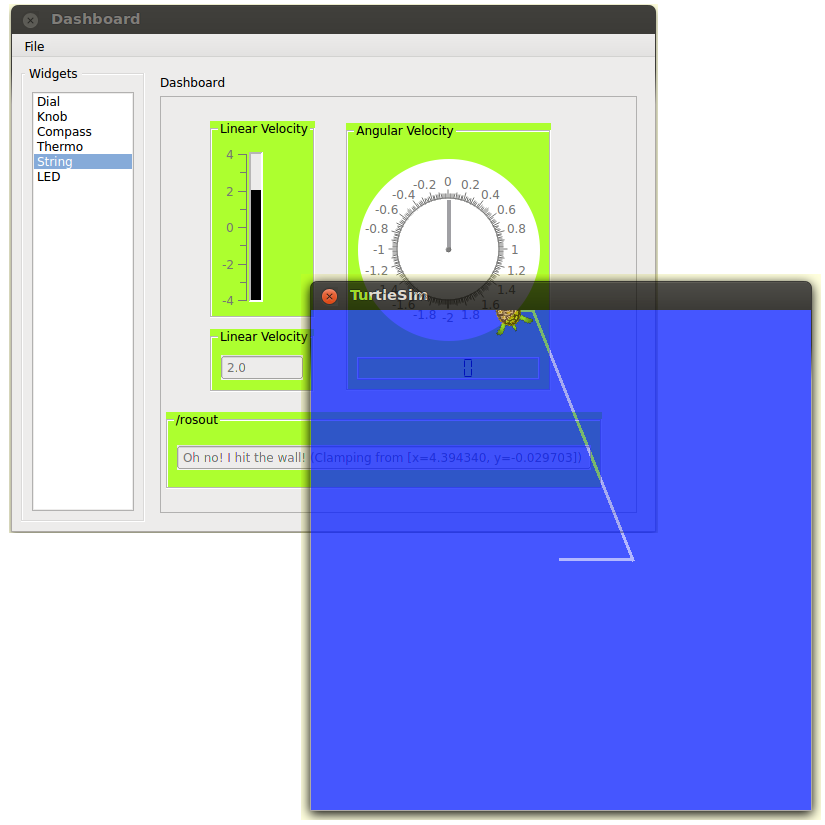
\includegraphics[width=0.9\textwidth]{img/showcase3.png}
  }  
  \caption{ROSDashboard running alongside turtlesim\_node.}
  \label{showcase}
\end{figure}

Figure~\ref{rosgraph_simple} shows the ROS computation graph during the execution of the showcase scenario. It shows how ROSDashboard is connected to the nodes which are debugged. The topics needed for the showcase are \emph{/turtle1/command\_velocity} for the linear and angular velocity and \emph{/rosout} for warnings when the turtle hit the wall.

\begin{figure}[thpb]
  \centering
  \framebox{
    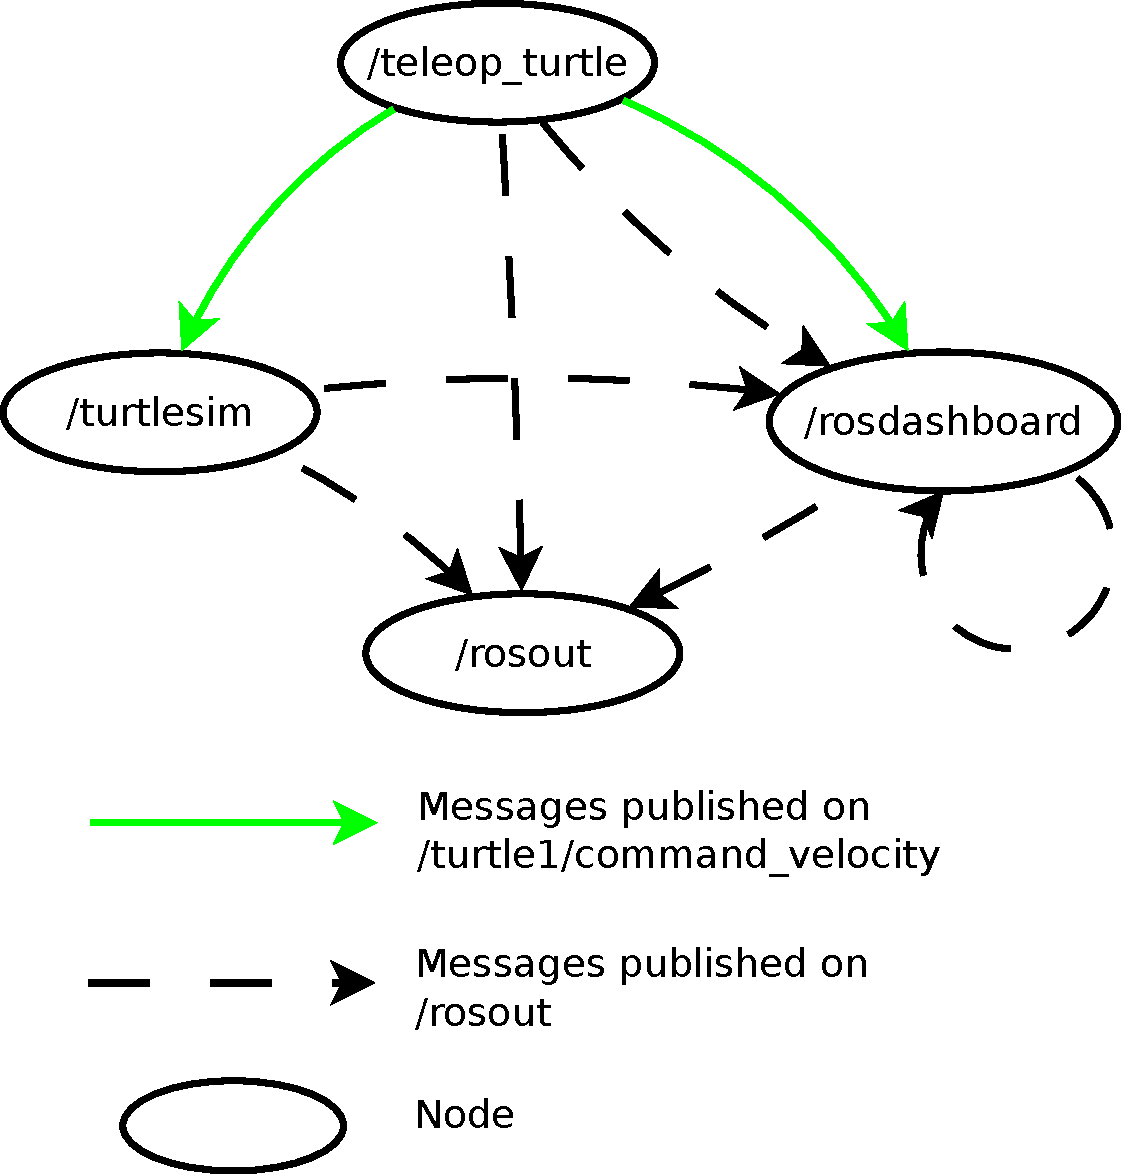
\includegraphics[width=0.7\textwidth]{diagrams/rosgraph}
  }  
  \caption{Simplified ROS computation graph with ROSDashboard.}
  \label{rosgraph_simple}
\end{figure}

\section{Adding New Widgets}
\todo{this could be a good spot for the section from the previous chapter about the plot widget}

\section{Nao Showcase}
A recent problem during the development of an existing project was chosen as use case \comm{showcase? case study?} to evaluate \q the use of ROSDashboard during the debugging of a robot. The project's goal is to use the Nao Robot \comm{cite} together with ROS to follow people and engage in conversations with people.

\todo{introduce nao and choreograph}

To move the head towards the person talking to the Nao Robot, a sound location algorithm is used. The sound location algorithm is already built in to the Nao Robot and can be accessed using ROS topics. The algorithm publishes the location where the sound comes from as a triplet of the horizontal location, vertical location and confidence. When the algorithm was used in the "Sound Tracker" module in Choreographe \comm{cite} to move the head of the Nao Robot it sometimes oriented the head to a random direction unrelated to the real direction of the sound source.

The developer of this system tried to find out whether the problem lies with the accuracy of the sensor, the implementation of the sound location algorithm or the "Sound Tracker" module moving the head. Since the data from the sound source is published as a triplet of numbers, debugging the problem by looking at numbers in a console was a problem. ROSDashboard was used to visualize the values from the sound location algorithm to determine where the problem of wrong head positions lies.

% case study configuration
\todo{find out how nao runs ros, describe where the master was, where the visualization was running} \cite{Cousins2010}

\todo{append saved dashboard json in appendix}


% Since to Nao Robot sometimes moved the head to a neutral position and looked up, either a error in the sensory input or in the sound location algorithm was suspected.

This showcase \q shows how the sound location algorithm was debugged with and without the use of a visualization tool.

%The first section presents the experimental setup and software configuration.
\todo{write about the configuration of the experiment: nao running with connection to the router, desktop machine running the clap orientation detection, laptop running with the dashboard}

\todo{Introduce the example: the goal is to track the orientation of a sound with the nao robot. During initial experiments with the shipped programming environment (choreography) some "weird" behaviour was noticed: sometimes the robot could not locate the noise and the head looked straight up. To investigate whether this is a bug in the algorithm or a sensor problem, the data has been visualized in rosdashboard}

\todo{show screenshot of the console with orientation data from print statements, show rxbag with raw message values (???), show rosdashboard with the visualization: compass gives direction of the sound based on the position of the nao, thermo widget gives altitude, thermo with confidence??}

\subsection{Case Study Configuration}
\todo{is this important? drop}
\todo{old structure}
What machines, software versions, robots, etc were used.

\subsection{Discussion}
Discuss the results from the case study?
